\chapter[SID]{SID}
--------------------- FALAR SOBRE O SID

\section{Visão Geral}
O SID está estruturado em duas vertentes, o WEB e o \textit{mobile}, ele foi desenvolvido com o objetivo de oferecer uma aplicação de divulgação que possua integração com as redes sociais de forma ágil, intuitiva, dinâmica e amigável para os administradores e para os usuários comuns, além de melhorar a efetividade do processo de disseminação das informações referentes ao Campus. Atendendo ao objetivo principal, onde é divulgação de informações através de uma plataforma WEB e \textit{mobile}.

Necessitando sempre do uso da rede para realizar atualizações, o SID está dividido em três módulos, o primeiro deles é o administrador, onde é possível fazer o gerenciamento completo do conteúdo que será apresentado no segundo módulo chamado cliente, nesse segundo módulo será apresentado as informações que foram cadastradas no módulo administrador, onde então serão propagadas por monitores ou celulares. O terceiro módulo é o \textit{mobile}, onde o usuário poderá ter acesso a todas as divulgações assim como no módulo cliente, mas com o incremento de troca de mensagens entre professores e alunos. 

A divisão de módulos foi feita para que seja possível atender a arquitetura cliente-servidor, ela mostrou-se necessário para minimizar o processamento nos outros dois módulos, centralizando o processamento das informações em um sistema mais robusto, ficando a cargo do outros módulos somente exibir as informações recebidas e realizar pequenos processamentos.

O sistema WEB foi desenvolvido na linguagem PHP, usada para estruturação do projeto, a linguagem JavaScript para realização das requisições de trocas de informações entre os módulos e as linguagens HTML e CSS para desenvolvimento das telas do sistema para os três módulos. Usa-se também o Banco de dados PostGreSQL, para armazenamento das informações localmente e que os dados sejam persistentes.

Baseado em desenvolvimento ágil, com metodologia SCRUM, foram definidos sprints semanais, comumente marcada as quartas feiras, para definição das funcionalidades a serem desenvolvidas ou melhoradas. Essa metodologia se torna importante para que o progresso seja acompanhado em cada parte do seu desenvolvimento.

No desenvolvimento, foram usados alguns \textit{framework}, O primeiro deles, usado em conjunto com o PHP, foi o ZEND que tem a finalidade de estruturar o código em modelo, visão e controle. Outro \textit{framework} foi o Doctrine, usado para efetivação da comunicação entre o banco de dados e a orientação a objeto. Foi usado também o Framework7 (F7), em conjunto com o Cordova, para que fosse possível o desenvolvimento do modulo mobile.  

\section{Modulo Administrador}
Com o uso da estrutura cliente-servidor, esse modulo é responsável por conceder ao usuário administrador a funcionalidade de gerenciar todas as informações do sistema podendo inserir, alterar, e retirar as divulgações, ou seja, fazer todo o gerenciamento das informações que são repassadas ao módulo cliente e \textit{mobile}.

O sistema de autenticação escolhido foi a login com o Facebook, ferramenta que a própria rede social disponibiliza. Optou-se por ele não somente pela segurança, por ser baseado em sistemas criptográficos, mas também porque algumas funcionalidades do sistema dependem de dados que são recuperados após o processo de autenticação.

Os elementos presentes no módulo e suas funcionalidades são descritas abaixo: 

\begin{enumerate}
   \item Legenda: É um campo de texto destinado a informação a ser repassada de forma sucinta e clara ao usuário final por intermédio cliente ou mobile. 
   \item Texto: É todo o texto que será enviado ao Facebook, contendo informações como descrição da publicação, data e horário da realização e um possível \textit{link} para acesso a mais informações. 
   \item Data de Início: É a data inicial em que o publicação começará a ser exibida no cliente e no mobile.
   \item Data de Término: É a data final em que o publicação deixará de ser exibida no cliente e no mobile.
   \item Imagem: Será a imagem enviada para o Facebook, para o cliente e para o mobile. Essa imagem pode ser um \textit{banner} de apresentação de um evento, por exemplo.
 \end{enumerate}

A Figura \ref{fig:administrador1}, consiste em representar como os elementos supracitados são inseridos a partir da visão do operador do sistema no módulo administrador. O diagrama de sequência para esta funcionalidade encontra-se na imagem \ref{fig:diagrama1}
 
\begin{figure}[H]
\centering
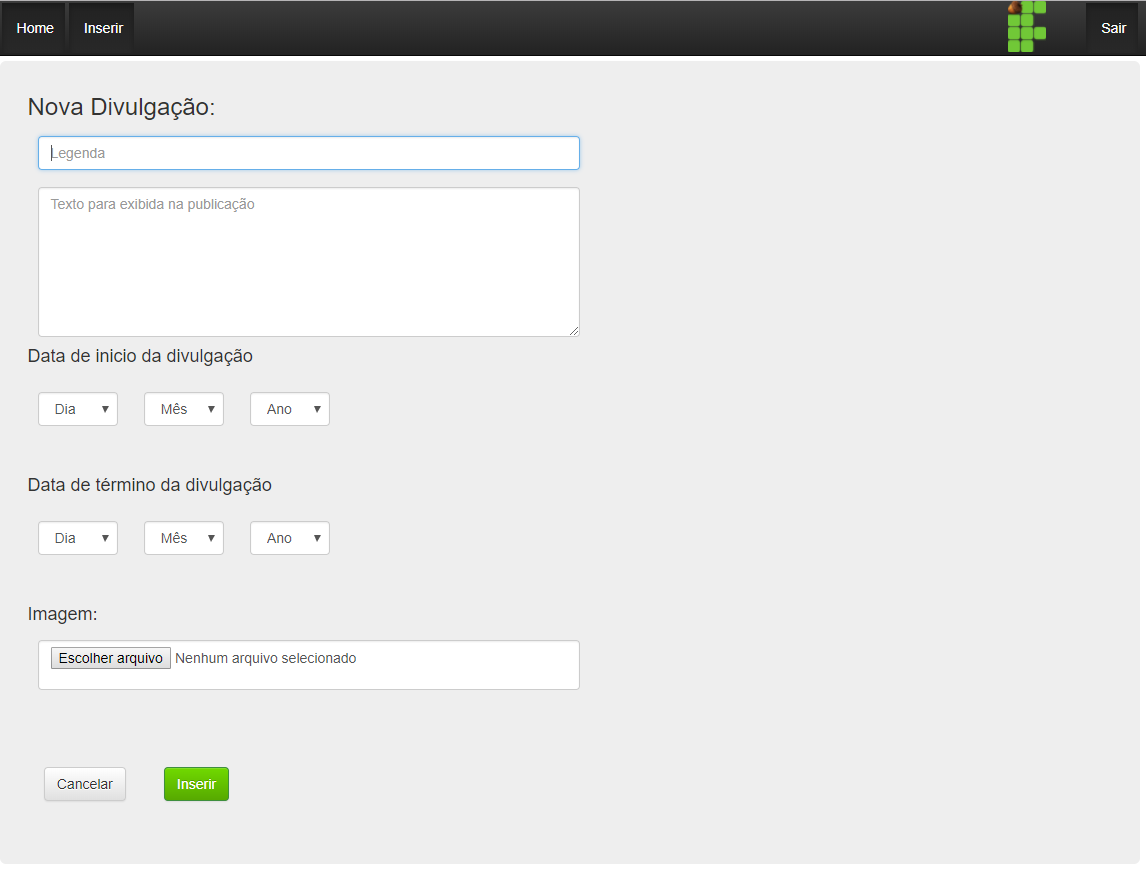
\includegraphics[scale=0.5]{figuras/administrador1}
\caption{Página de inserção no módulo administrador.}
\label{fig:administrador1}
\end{figure}

\maxwell{COLOCAR DIAGRAMA DE SEQUENCIA}

\maxwell{FALAR SOBRE OS CAMPOS E SUAS LIMITAÇÕES}

O campo imagem é repassado para a API como parâmetro \textit{source}, já o campo texto da publicação é repassado como \textit{messagem}. Todos os campos são de preenchimento obrigatório, entretanto, somente os campos imagem e texto da publicação são enviados ao Facebook. Os outros campos não são enviados a rede social, ficam armazenados apenas no banco de dados.

Se durante o envio alguma das transações não forem efetivadas, será retornado a mensagem de erro, assim como retornará a mensagem de sucesso, caso não ocorra nenhum erro.

\section{Modulo Cliente}
O modulo cliente tem a função de apresentar as divulgações de maneira atrativa, intuitiva e dinâmica para o usuário. A estrutura e organização do que será apresentado, está disposto na  figura \ref{fig:cliente1}.

Os elementos que compõe a página que será apresentada, são dividos em cinco itens, que estão descritos abaixo.

\begin{enumerate}
   \item Imagem: O conteúdo, poderá ser apresentado como uma imagem estática ou como GIF (imagem com animação), não oferecendo suporte a vídeos, até o momento, mas que poderá ser implementado em versões futuras. 
   \item Legenda: A legenda é apresentada em movimento linear da direita para a esquerda, possibilitando a leitura de forma dinâmica de toda a frase.
   \item QR Code: Imagem, que por meio de uma aplicativo celular, possibilita a leitura que contem o \textit{link} de acesso a publicação publicada na rede social Facebook.
   \item Horário: Relógio que apresentará a data e hora atual.  
   \item Comentários: Espaço que será apresentado comentários publicados e devidamente moderados.
 \end{enumerate}
  
\begin{figure}[H]
\centering
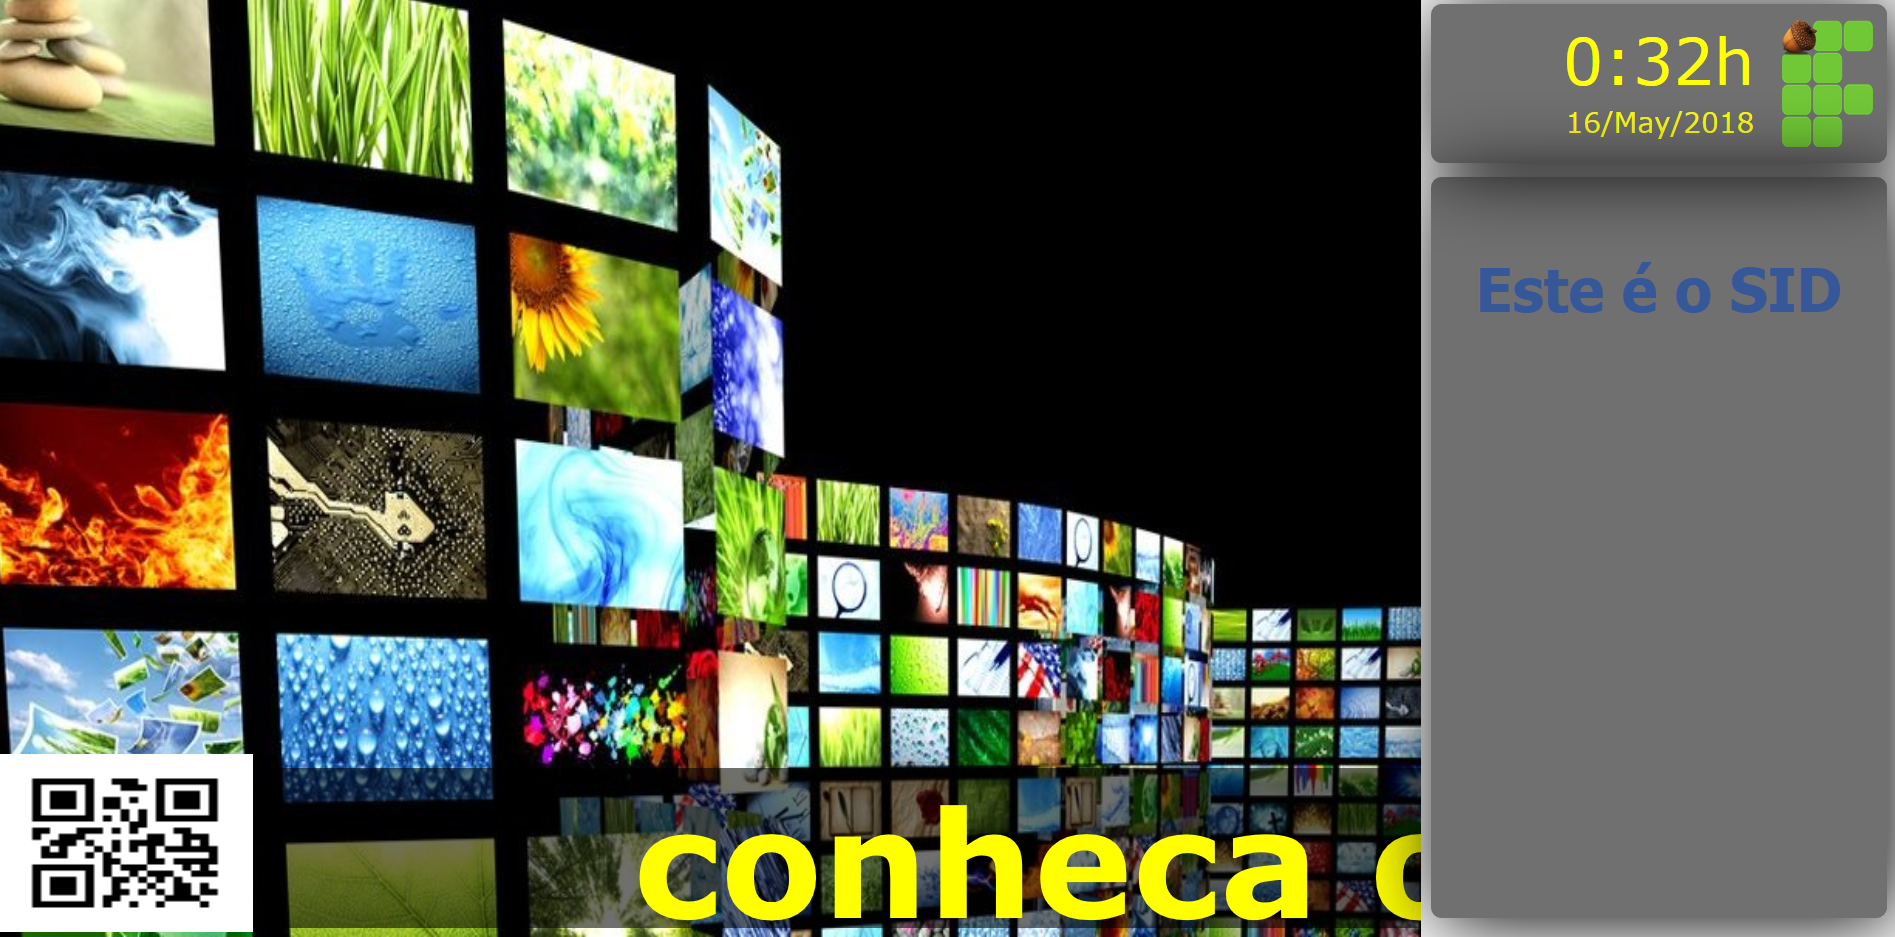
\includegraphics[scale=0.3]{figuras/cliente1}
\caption{Página do cliente}
\label{fig:cliente1}
\end{figure}

Usando Javascript com suporte a biblioteca JQuery, o módulo cliente efetua uma requisição ao servidor que receberá como resposta um JSON, contendo o número de posições equivalentes ao número de publicações válidas. Cada posição desse JSON terá três variáveis, são elas: 'bd','comentarios' e 'imagem'. 

A 'bd', contém uma \textit{array} de duas posições, contendo 2 \textit{string}, sendo elas o legenda e link, esses dados foram armazenados pelo servidor no banco de dados, na criação da publicação. A 'comentarios' é um array de \textit{string} que pode possuir zero ou mais itens, cada item representa um comentário na publicação, onde cada item possui a data da criação, quem fez, a mensagem, a foto e o id do comentário. Já a 'imagem' é uma \textit{string} de é um arquivo codificado em base64, que será descodificado pelo módulo.

O conteúdo recuperado da variável 'bd', será apresentado nos itens 2 e 3, respectivamente. Já o conteúdo recuperado da variável 'comentarios' será apresentado no item. Enquanto os da variável 'imagem', será descodificado e apresentado em forma de imagem no item 1.


\maxwell{FALAR MAIS SOBRE AS PARTES (qrcode, legenda, comentários)}

\section{Modulo Mobile}
O \textit{mobile} é responsável por apresenta as divulgações e disponibilizar a possibilidade de troca de mensagens entre professores e alunos que possuam um login e senha. 
Figura \ref{fig:mobile1}

\maxwell{FALAR SOBRE O MODULO}
 
\begin{figure}[H]
\centering
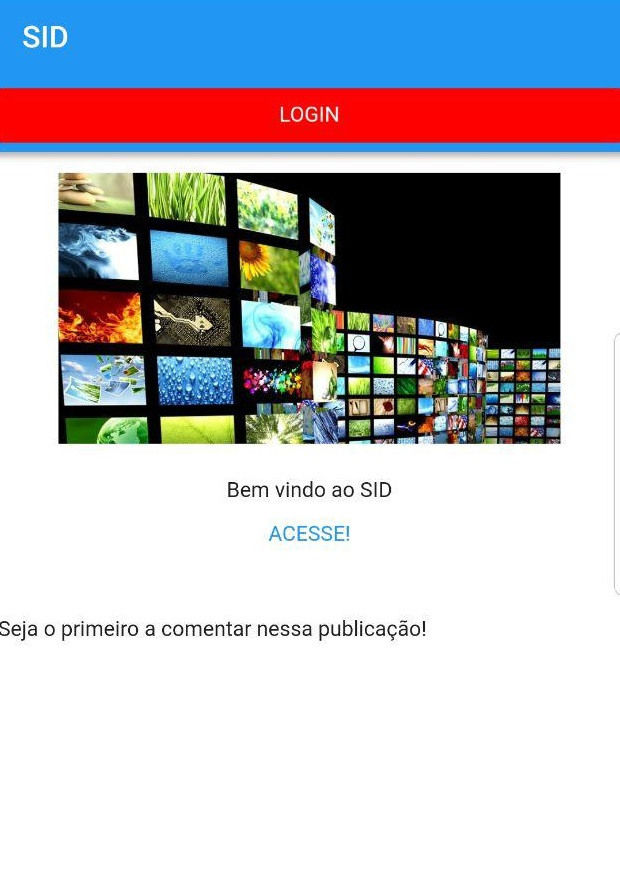
\includegraphics[scale=0.6]{figuras/mobile1}
\caption{Página de inserção no módulo administrador.}
\label{fig:mobile1}
\end{figure}

\maxwell{FALAR SOBRE OS BOTOES}

\section{Arquitetura}
\begin{figure}[H]
\centering
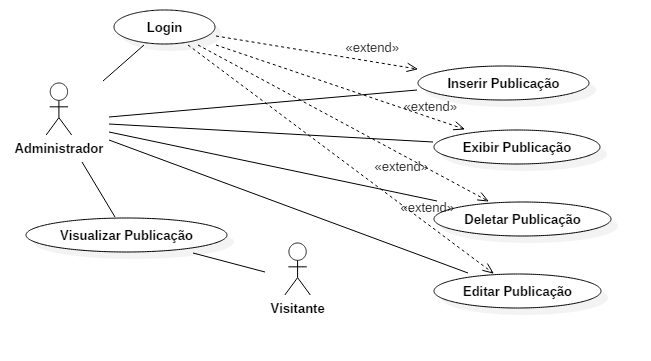
\includegraphics[scale=0.6]{figuras/casosDeUso}
\caption{Casos de uso da ações dos módulos administrador e cliente}
\label{fig:casosDeUso}
\end{figure}

\maxwell{COLOCAR DIAGRAMA DE CLASSES}

\maxwell{COLOCAR DIAGRAMA DE SEQUENCIA}

\maxwell{COLOCAR MODELO ENTIDADE RELACIONAMENTO}

\section{Integração}
Para acesso a funções restritas do sistema é necessário que um \textit{login} seja feito. Para isso, é utilizado a ferramenta de \textit{login} do Facebook, ela oferece um botão para ser colocado na página, esse botão tem a finalidade de iniciar o processo de login, após ser clicado é feito a chamada do método ''getRedirectLoginHelper``, onde é passado as informações de permissões que serão necessárias e o endereço de callback, que será a página de retorno caso o processo seja efetivado. O endereço de callback deve ser o mesmo informado no aplicativo criado na página da rede social.

Após o login, as informações usadas são guardadas na sessão do usuário, para usos posteriores, além disso, todo o processo de armazenamento de informações, envios ao Facebook e retornos de solicitações não devem ser visíveis ao usuário. 

Qualquer divulgação inserida na pagina do SID no Facebook utiliza-se do nó “photo”, ou seja, a divulgação que o SID repassa à Graph API contém a mesma estrutura de uma imagem postada por um usuário convencional desta rede social.

A Figura \ref{fig:imgfacebook1} apresenta como ficará uma publicação no Facebook após o uso do SID para criação da mesma. Nela é apresentado informações como quem realizou a publicação, o texto e a imagem que foram informados durante a criação da divulgação pelo SID.

\begin{figure}[H]
\centering
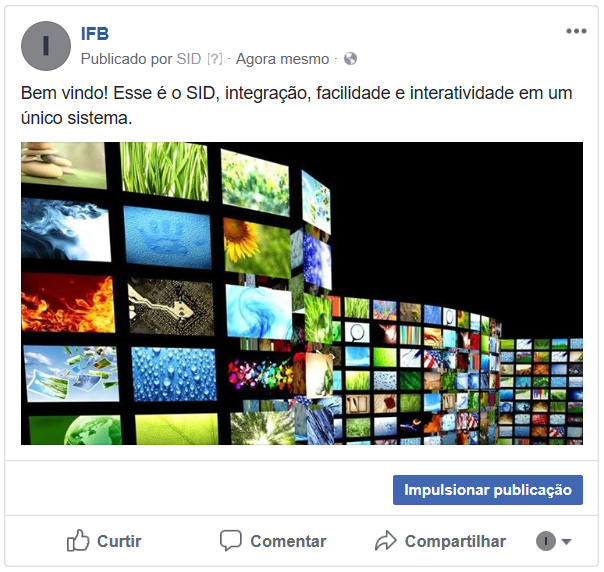
\includegraphics[scale=1]{figuras/imgfacebook1}
\caption{Divulgação enviada ao Facebook com auxilio do SID}
\label{fig:imgfacebook1}
\end{figure}

Com o uso do método \textit{post} em conjunto com a Graph, a rede social recebe os parâmetros e faz a criação de um novo objeto, criando uma nova aresta que terá como vértice a publicação e a página. O retorno da requisição é o id desse novo vértice criado. 





\maxwell{Para criação de um novo vértice são obrigatórios algumas permissões, os mesmos do usados no login, com adição do: id\underline{{ }}pagina e do \textit{token}. 

\begin{itemize}
\item O \textit{token} é um conjunto de caracteres que identifica para o Facebook as autorizações que a aplicativo possui.

\item O id\underline{{ }}pagina é o identificador único da sua página ou perfil.
\end{itemize}

É possível também solicitar dados referentes a postagens efetivadas. Para isso é necessário a passagem de alguns parâmetros no método ''get`` e a Graph. Assim como no ''post``, o ''get`` usa todos os parâmetros com exceção do id\underline{{ }}pagina, onde será informado o id\underline{{ }}publicação em substituição do da página.}

\section{Possível solução para Implementação - Rapberry}
Desde a sua invenção em 1971, microprocessadores vem sendo usados no desenvolvimento dos mais variados tipos de eletrônicos ou outros equipamentos, substituindo até mesmo sistemas mecânicos. Algo que vai além de um simples software, os microprocessadores devem ser capazes controlar as ações de um dispositivo. \cite{rosenstark2007}

Para \cite{aristotelous2016}, o objetivo essencial de todos os tipos de empresa é a rentabilidade, podendo ela ser alcançada usando uma solução de baixo custo, boas tecnologias e com um preço atrativo. Teste do \cite{aristotelous2016} apresenta a possibilidade de se ter um servidor completamente funcional com sistema operacional Linux por um equipamento de 35\$, possibilitando a criação de um servidor, por exemplo de um repositório na nuvem com um baixo custo, flexibilidade e eficiência energética. 

Grandes servidores oferecem um melhor desempenho, entretanto, o baixo uso, a pouca eficiência energética ou até mesmo o pouco espaço podem limitar o uso desse tipo de equipamento. Nesse sentido, para \cite{cusick2014}, placas de circuito oferecem vantagens como o uso de pouco espaço, desempenho significante com baixo custo e consumo, além do suporte a diversas soluções de software oferecendo múltiplas opções de interface com uma variante do Linux. 

\section{Visão Geral}

\maxwell{O Facebook oferece diversos produtos para incorporar ao aplicativo externo, entre eles está o de login do Facebook. Esse produto oferece ao desenvolvedor a possibilidade de oferece ao usuário do aplicativo uma ferramenta de login usando as credenciais do Facebook.

A autenticação (\textit{login}) no módulo administrador é feita usando a ferramente de login oferecida pela rode social, então para acesso é necessário um usuário cadastrado no Facebook e cadastrado no no banco de dados do SID. O uso de um usuário vinculado a rede social se torna necessário pois existe a necessidade da página apresentar qual o perfil está realizando a ação, além da necessidade de moderação dos comentários que serão exibidos. 

Para autenticação e efetivação de todas as requisições feitas pelo aplicativo para o Facebook, seja ela para requisitar informações das publicações ou realizar uma nova publicação, é usando um \textit{token} de acesso, que é obtido após a efetivação de login do usuário com o Facebook. O \textit{token} é uma cadeia de caracteres que identifica um usuário, aplicativo ou página, identificando a sessão. Em cada nova requisição a rede social, o \textit{token} será usado, se autorizado, pela aplicação para permitir o envio de requisições HTTP usando seus identificadores únicos, recebendo a respectiva resposta.}

\section{Elementos Usados}
Para publicação no perfil pessoal, a Graph API requisita duas permissões, sendo a “email”, onde é requisitado o acesso ao endereço de email do usuário para que seja possível a autenticação do SID com o Facebook e a “publish\underline{{ }}actions”, onde fornece acesso a realização de publicações em nome da pessoa que está usando o aplicativo \cite{facebook2018a}.

Como o SID será usado em uma página e não em um perfil pessoal, duas novas autenticações se tornaram necessárias, sendo a “manage\underline{{ }}pages”, usada para recuperar as permissões de acesso a pagina e a “publish\underline{{ }}pages”, usada parar permitir que aplicativos publiquem na página \cite{facebook2018a}.

Usando o identificador único da foto é possível recuperar informações das arestas, que são informações como a URL, comentários e curtidas. Esse recurso é utilizado para recuperar o endereço da publicação, os comentários e curtidas que serão apresentados respectivamente nos campos destinados ao QRCode e na coluna de comentários do módulo cliente.

Na criação de uma nova publicação, usando o SID, são passados para a Graph API dois parâmetros para inserção, o primeiro deles é “message”, onde será passado o texto que será exibido na publicação e o outro é “source”, onde será passado a imagem para ser exibida juntamente com o texto. Para envio de imagem para a rede social, é necessário passar na imagem como parâmetro o método “fileToUpload”. 

Alguns dos elementos que são solicitados pela aplicação na criação de uma nova publicação, são omitidos no envio para o Facebook, pois esses dados serão usados apenas para serem armazenados no banco. Os elementos omitidos são os campos data de inicio, a data de termino e a legenda. 

------------------ CONTINUA  P48-------------------